\chapter{Experiment}

\section{Energy loss in material}
The average energy loss in a material can be described by the Bethe-Bloch equation,
\begin{equation}\label{eq:bb}
\frac{dE}{dx} = \frac{4\pi NZ^2e^4}{mc^2\beta^2} (ln \frac{2mc^2\beta^2\gamma^2}{I} - \beta^2).
\end{equation}
Where $N$ is the number density of electrons in the medium, $e$ the elementary charge, $mc^2$ is the rest mass of the electron, $Z$ is the charge of the traversing particle, $I$ is the mean excitation energy of the medium, and $\beta$ is the velocity of the particle. There is a large variation in energy loss around this mean value, with a long high energy loss tail. A full description of the energy loss distribution can be described in CITE HERE.


\section{Pad Response Function}
The charge distribution on the pad plane resulting from an electron avalanche is two dimensional, as illustrated in Fig.~\ref{fig:prf}, with the projections onto the $x$ and $z$ axis of this distribution labeled as $\rho(x)$ and $\rho(z)$ respectively. The charge observed on each pad is the integral of this distribution over the pad's dimensions, which is called the Pad Response Function (PRF).

In this example the clustering direction would be along the $x$ axis, as illustrated by the bolded pads. By choosing to cluster only in one direction, we have not included the charge in adjacent pads along the $z$ axis resulting from the tails of $\rho(z)$. Therefore the charge not included in the the bolded pads will be incorporated into adjacent clusters, introducing small correlations in charge between neighboring clusters. 


\subsection{Gatti Pad Response Function}
Gatti \cite{gatti} derived a semi-empirical formula for the charge distribution in a simple multi-wire TPC. The function given in Eq.~\ref{eq:gatti}, depends only on the width of a pad ($w$), the distance of the anode plane to the pad plane ($h$), and the distance of the pad center to the avalanche point $\lambda$. It is a single parameter equation where the two parameters $K_1 = \frac{K_{2}\sqrt{K_3}}{4 \arctan(\sqrt{K_3})}$ and $K_2 = \frac{\pi}{2}\left(1-\frac{\sqrt{K_{3}}}{2}\right)$ depend on the parameter $K_3$, which is a function of the ratio of the anode wire diameter to the distance of the anode wires to the pad plane. $K_3$ can be looked up in a graph in \cite{blumrol} and \cite{gatti}.

\begin{equation}\label{eq:gatti}
\begin{split}
PRF_{\mathrm{Gatti}}(\lambda)
& = \frac{K_{1}}{K_{2}\sqrt{K_{3}}}\bigl[\arctan(\sqrt{K_{3}}\tanh\bigl[K_{2}\bigl(\frac{\lambda}{h}+\frac{w}{2h}\bigr)\bigr]) \\
& - \arctan(\sqrt{K_{3}}\tanh\bigl[K_{2}\bigl(\frac{\lambda}{h}-\frac{w}{2h}\bigr)\bigr])\bigr] \\
\end{split}
\end{equation}

\subsection{Experimental Pad Response Function}

The correlations we introduced by only clustering along one direction do not play a significant role in the particle identification, but cause deviations from the expected Gatti distribution. Also, analytic PRFs only exist for classical multi-wire TPCs. For these reasons it is useful to experimentally measure the PRF and fit it with an empirical function, typically a Gaussian, to describe its behavior. 

As in Fig.~\ref{fig:topview}, we postulate that the PRF is a function of the total charge deposited in a cluster $Q = \sum_i q_i$, and the difference in position of the center of the $i^{th}$ pad, $x_i$, to the mean position $\bar{x} = \sum_i x_i q_i/Q$, defined as $\lambda_i = x_i-\bar{x}$. The PRF is simply defined as the charge fraction of each pad as a function of $\lambda$, as shown in Equation \ref{eq:prf}. 

\begin{equation}\label{eq:prf}
PRF(\lambda_i) = \frac{q_i(\lambda_i)}{Q}
\end{equation}

Averaging over many events in the experimental data, the resulting PRF for the S$\pi$RIT TPC is shown in Fig.~\ref{fig:expprf}. Here we see the deviations from the expected analytic Gatti distribution (black curve), whereas fitting with a two parameter Gaussian function (red curve) gives a better description of the  data, Eq.~\ref{eq:gaus}, with the two parameters being the normalization coefficient, $N_0$, width $\sigma$, and with a mean value assumed to be 0.

\begin{equation}\label{eq:gaus}
PRF_{\mathrm{Gaus}}(\lambda) = N_0 e^\frac{-\lambda^2}{2\sigma^2}
\end{equation}

\begin{figure}[ht!]
\begin{overpic}[width=\linewidth]{expprf}
\put(61,55){\contour{white}{ PRF${}_{\mathrm{Gaus}}(\lambda)$ eq. \ref{eq:gaus}  }}
\put(61,49){\contour{white}{ PRF${}_{\mathrm{Gatti}}(\lambda)$ eq. \ref{eq:gatti} }}
\end{overpic}
\caption{Experimental pad response function of many events for a crossing angle of $85^{\circ} < \theta \leq 90^{\circ}$.  }
\label{fig:expprf}
\end{figure}

\section{Pad Response Function vs. crossing angle}
The shape of the PRF depends on the crossing angle of the track \cite{gatti}. Plotted in Fig.~\ref{fig:prfangle} is the PRF of $\pi^-$ tracks vs. the crossing angle $\theta$. The PRF gets wider starting from $90^{\circ}$  and going to $45^{\circ}$; if we did not switch clustering directions the PRF would become wider until it was a uniform distribution and there was no position resolution. Since we switch the clustering direction from $x$ to the $z$ direction at $45^{\circ}$, the opposite trend is seen where the PRF becomes narrower as the position resolution gets better going from $45^{\circ}$ to $0^{\circ}$.

\begin{figure}[ht!]
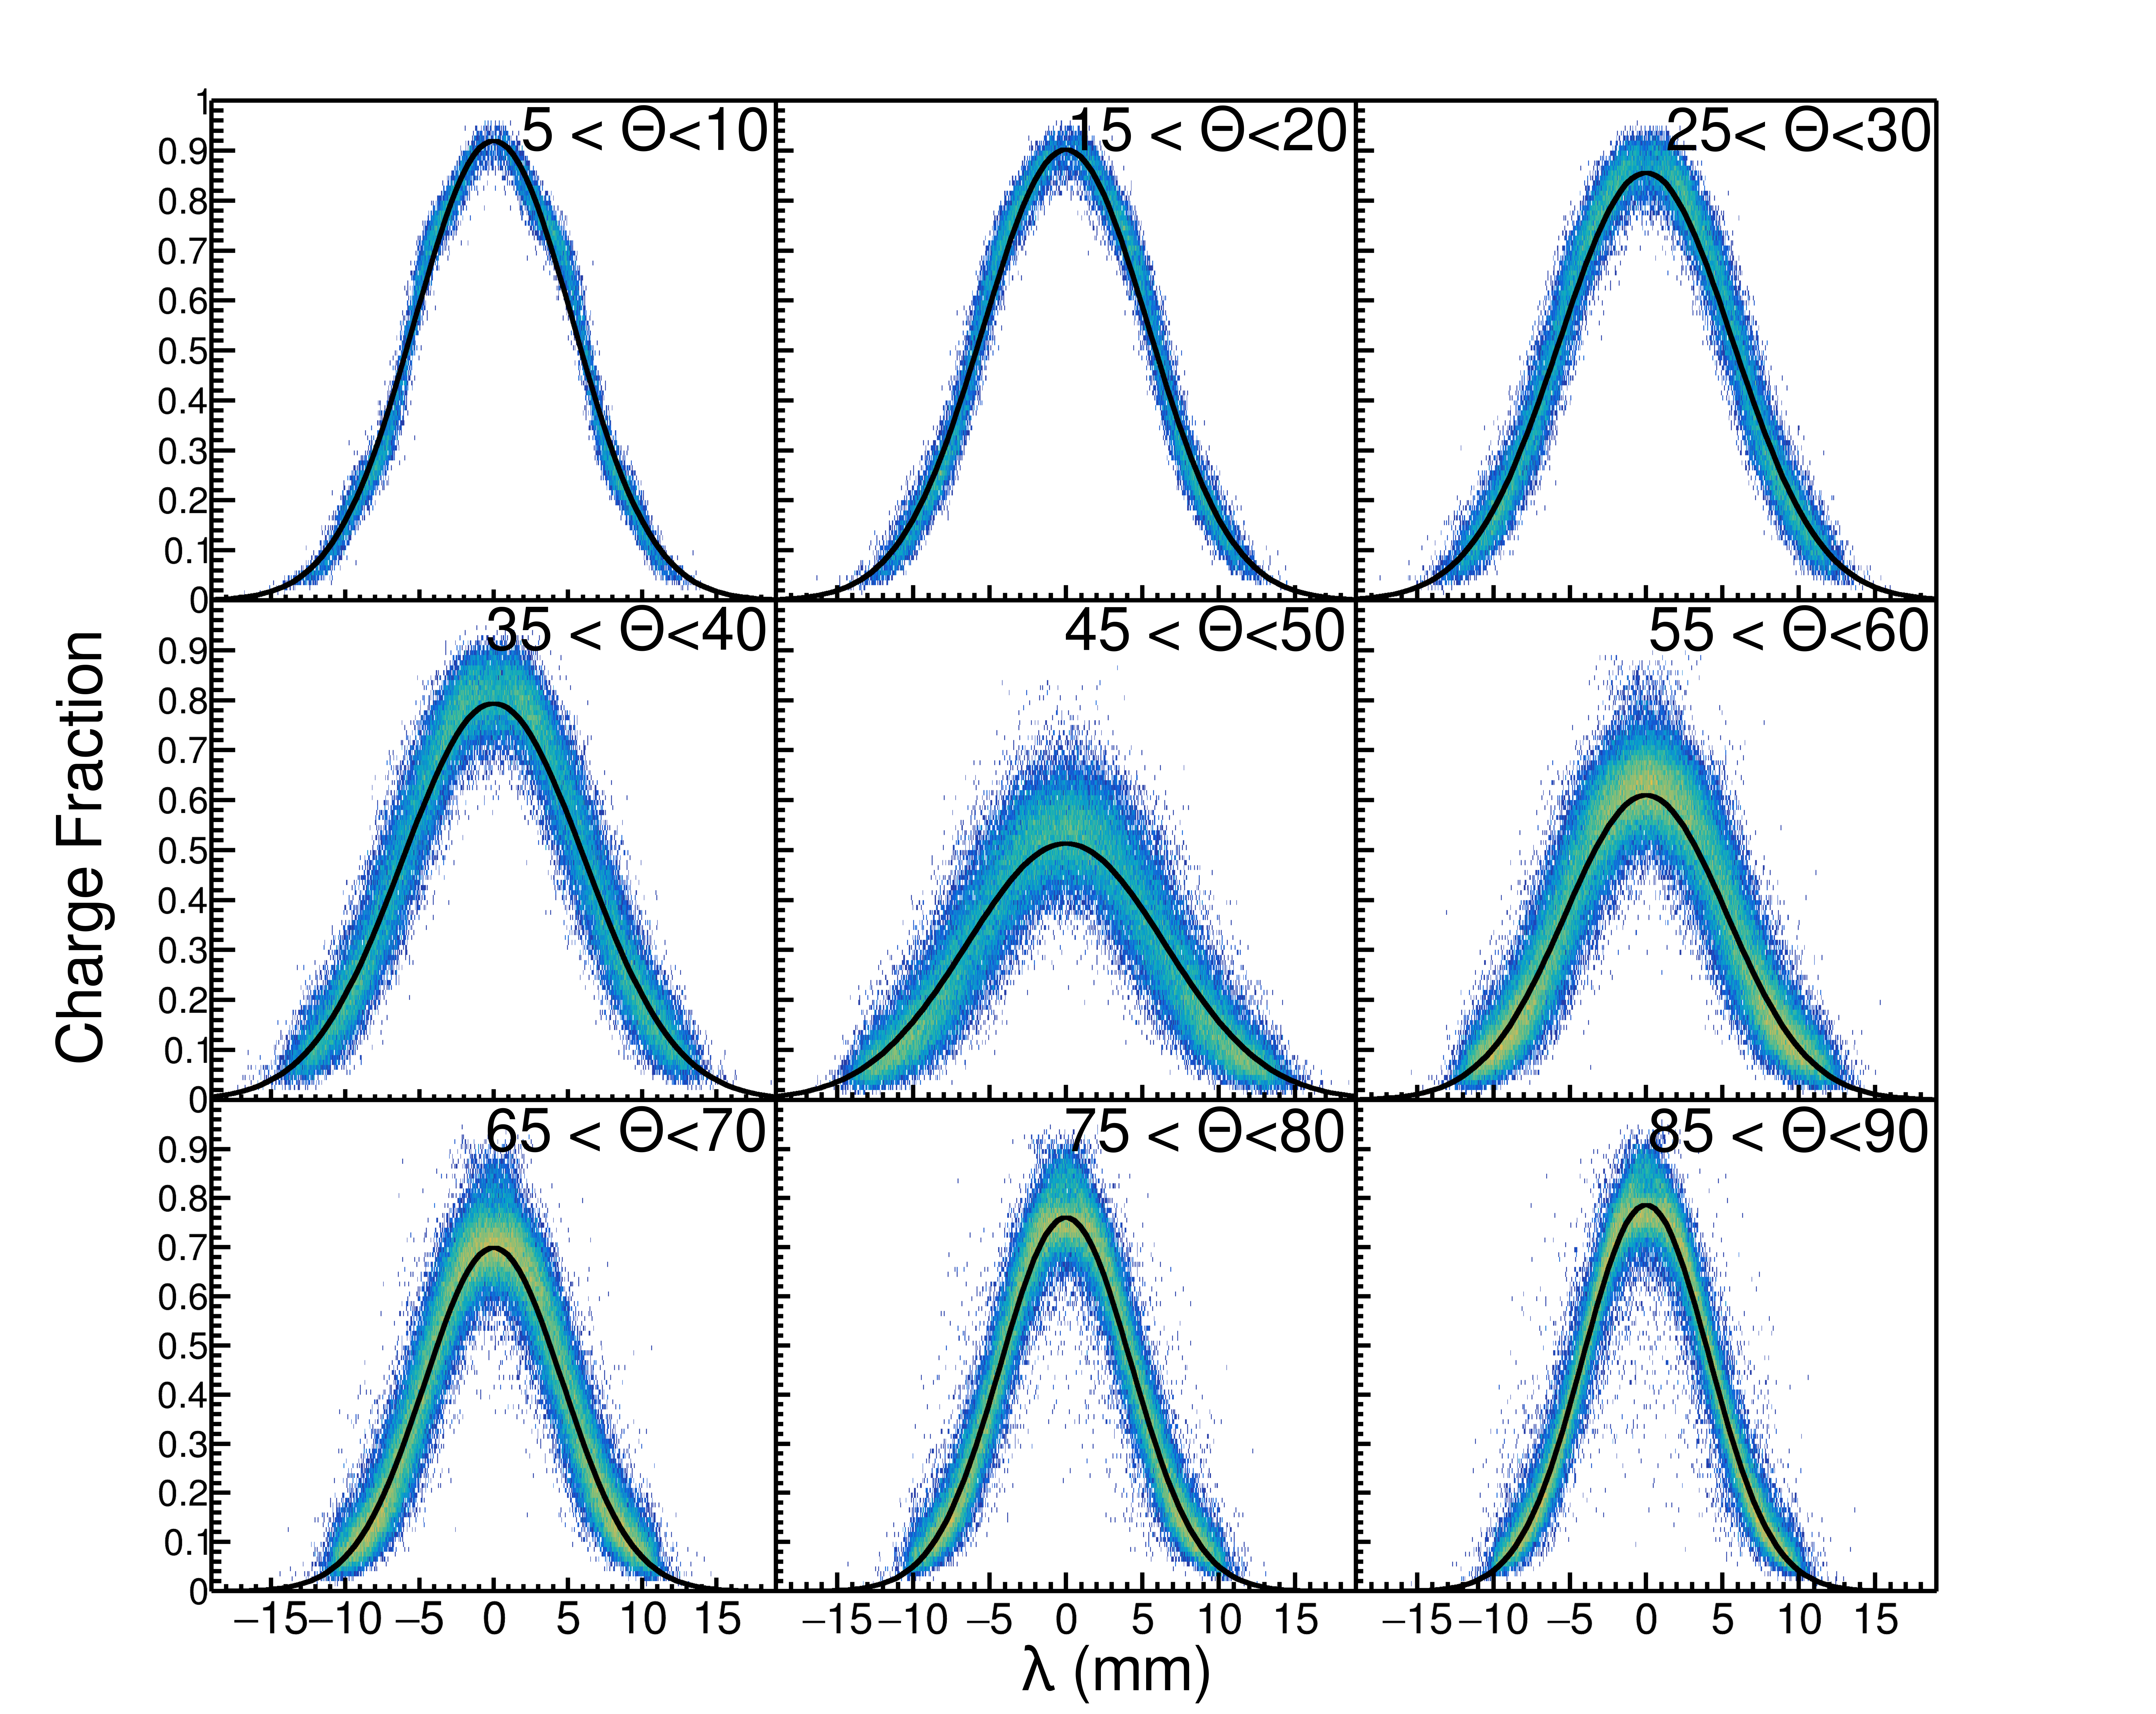
\includegraphics[width=\linewidth]{PRF_vsAngle}
\caption{Experimental pad response function as a function of the crossing angle $\theta$ with the corresponding fits.}
\label{fig:prfangle}
\end{figure}


\begin{figure}[ht!]
\begin{overpic}[width=\linewidth]{normsigma}
\end{overpic}
\caption{Parameters $N_{0}$ and $\sigma$ as a function of the crossing angle $\theta$ with the $4^{th}$ order polynomial fits.}
\label{fig:normsigma}
\end{figure}

\begin{comment}
\begin{table}
\centering
 \begin{tabular}{||c c c c c c||} 
 \hline
 Coefficient & $c_0$ & $c_1$ & $c_2$ & $c_3$ & $c_4$ \\ [0.5ex] 
 \hline\hline
 $0 < \theta < 45$ & & & & &  \\ [.25ex]
 \hline
 $N_0$ & .897 & 5.766E-3 & -4.263E-4 & 7.444E-6 & 5.705E-8 \\ 
 \hline
 $\sigma$ & 5.496 & -3.920E-2 & 2.693E-3 & -5.208E-5 & 5.334E-7\\
 \hline
 $45 < \theta < 90$ & & & &  & \\ [.25ex]
 \hline	
 $N_0$ & 1.220 & -6.258E-2 & 1.608E-3 & -1.492E-5  & 4.654E-8 \\
 \hline
 $\sigma$ & 31.368 & -1.109 & 1.779E-2 & -1.336E-4 & 3.940E-7\\
 \hline
\end{tabular}
\caption{Coefficients of the $4_th$ order polynomial fit to the Gaussian parameters $N_0$ and $\sigma$. The polynomial form is given as $c_0 + c_1 x + c_2 x^2 + c_3 x^3 + c_4 x^4$}
\label{tb:coeff}
\end{table}
\end{comment}
 
Fits were performed to the experimental data with  $5^{\circ}$ width bins from $0^{\circ} < \theta \leq 90^{\circ}$. The two parameters of the Gaussian fits are plotted versus $\theta$ in Fig.~\ref{fig:normsigma}; a $4^{th}$ order polynomial fit between these points allowed for interpolating between $\theta$.




\section{S$\pi$RIT TPC Overview}
Add Overview image with labels


The Samurai Pion-Reconstruction and Ion Tracker Time Projection Chamber (S$\pi$RI TPC) is a Multi-Wire Proportional Counter developed to measure pions and other light charge particles resulting from radioactive heavy ion collisions in a fixed target experiments.  The TPC is enclosed in a thin aluminum sheet walls all around in order to minimize neutron scattering and to allow for light charged particles to reach the arrays of scintillating bars detectors on the sides and downstream of the TPC. The S$\pi$RI TPC was developed to fit inside the Samurai dipole magnet used at the Rare Isotope Beam Factory (RIBF) at RIKEN in Wako-shi, Japan \cite{riken}; the dipole gap limited the vertical space of the TPC. More detail and specifications of the Samurai dipole magnet are given in \cite{samurai}. 

A target ladder allowed for up to 5 fixed targets to be mounted. A ACME worm gear allowed for the x-axis motion for changing the targets during the experiment, without needing to open or move the TPC. The motion of this worm gear was translated through the target motion feed-through by several brass gears and non-magnetic gear boxes. The motion of the target ladder could be controlled by hand or by operation of the drill. The targets were mounted on stand-offs on the target ladder and also had z-axis motion. This allowed for the targets to be positioned as close as possible to the thin window of the field cage, maximizing the geometric acceptance. 

The electronics were mounted to the aluminum top plate. Several aluminum ribs were mounted to the top of the plate to bring structural rigidity. A flatness within 150$\mu$m was achieved across the whole top plate as measured by a laser position system. The charge sensitive pads of the pad plane were etched into several circuit boards were recessed and glued to the bottom portion of the top plate. Vias through the pad plane circuit boards brought the signal traces from the pads to surface mount pads on the other side of the boards. Several holes cut through the top plate allowed for the interface cables of the electronics to be connected to these surface pads. 

Just below the pad plane were a set of three wire planes; the gating grid, ground, and anode wire planes. The detailed function of these wires will be explained later but they served to separate the boundary between the drift volume and the avalanche volume. 

The front and sides of the field cage were assembled from 8 independent rigid circuit boards. The downstream window served as the downstream wall of the field cage all though it was was a large polycarbonate frame in which a removable kapton window could be installed. This thin window minimized the scattering of exiting neutrons and charged particles for downstream detectors. 

The voltage step down takes the high voltage of the field cage cathode and steps the voltage down through a set of copper rings and a resistor chain, minimizing the chance for sparking. 

\begin{table*}\centering
\ra{1.3}
\begin{tabular}{@{}rr@{}}\toprule 
\multicolumn{2}{c}{\spirit TPC Overview} \\
 \midrule
Pad plane area & 1.3 m x .9 m\\
Pad size       & 1.2 cm x .8 cm \\
Number of pads & 12096 (112 x 108) \\
Gas composition& 90\% Ar + 10\% CH${}_4$  \\
Multiplicity limit & 200  \\
dE/dx range        & Z=1-8, $\pi$, p,d,t,He,Li-O \\
Drift length       & 50 cm \\
\bottomrule
\end{tabular}
\caption{An overview of the properties of the \spirit TPC}
\label{tb:spiritoverview}
\end{table*}

\subsection{Enclosure}

\subsection{Voltage Step Down}

\subsection{Field Cage}

The field cage was designed to hang from the top plate and therefore needed to be of a lightweight construction. Also the materials needed to be thin to allow for light charged particle and neutrons to pass through without significant scattering for ancillary detectors. Therefore instead of a downstream wall, a large thin exit window was constructed. The cathode was constructed of an aluminum honeycomb laminate. Two sheets of ??? aluminum were bonded to a core of aluminum honeycomb structure providing a lightweight yet rigid structure for the cathode. 

\begin{figure}[H]
\includegraphics[width=\linewidth]{fc_explode}
\caption{Exploded view of the S$\pi$RIT TPC}
\label{fig:fc_explode}
\end{figure}

The field cage was constructed from several panels of printed circuit boards (PCBs). The epoxy in the common PCB substrate FR4 contains bromine which is not suitable for the long term operation of a TPC, as the bromine will eventually cause gain reduction of the wires [CITE]. The halogen free material chosen was Rodgers ????. We built the TPC with the option to run explosive gases such  hydrogen, thus we decided to have field cage an isolated volume from the rest of the TPC enclosure. While the risk of a high voltage spark was minimized using the voltage step down, the risk of sparking when using an explosive gas could be further minimized by isolating the detector volume from the enclosure volume thereby allowing you to run an insulating gas between the field cage while running the explosive gas inside the detector volume only.  

The front of the field cage was made of two PCBs and each side was constructed of three PCBs. The exit window was a 10$\mu$m thick Kapton window with evaporated aluminum strips on the inside and outside; mounted on a polycarbonate frame.

\subsection{Voltage Step Down}

To lower the risk of a high voltage spark around the cathode region a voltage step down was developed. A series of 7 concentric copper rings with 20 MOhm resistors between them steps the cathode voltage down to ground. This minimizes sharp transitions of the electric field and therefore sparking. 

\subsection{Wire Planes}
Add figure of gating grid transparency closed and open configuration 


\subsection{Pad Plane}
Add figure of close up of pad plane 

\subsection{Electronics}

Signals in the S$\pi$RIT TPC are amplified and digitized by the recently developed Generic Electronics for TPCs (GET) \cite{get}.  Short cables transmit the signals from the pads to the inputs of the AGET chips. Each AGET chip services 64 pads (63 pads are connected in our case), contains a pre-amplifier, and a Switched Capacitor Array (SCA), with a maximum of 512 time buckets with an adjustable sampling frequency of 1 to 100 MHz. Four AGET chips are mounted on one AsAd (ASIC and ADC) motherboard. The gain of each AGET can be configured as 0.12, 0.24, 1.0, or 10 pC over the whole dynamic range, and the ADCs on each AsAd board provides 12 bit resolution. The peaking times of the shaping amplifiers can be set to 69, 117, 232, 501, 720, or 1014 ns. In this experiment, the gain was set to the highest setting, 0.12 pC, the peaking time 117 ns, and the sampling frequency 25 MHz (resulting in 40 ns time buckets). The Aget 2.0, asad 2.1, and cobo 1.0 firmware versions were used. The variations in the electronics were calibrated by measuring the response of each channel to a injected reference pulse, covering the full dynamic range of each channel. 




\begin{table*}\centering
\ra{1.3}
\begin{tabular}{@{}rr@{}}\toprule 
\multicolumn{2}{c}{GET electronics settings}\\
\midrule
ADC bit range       & 14 bits \\
Sampling frequency  & 1-100 MHz \\
Dynamic range       & .12, .24, 1.0, 10pC \\
Peaking time        & 69,117,232,501,720,1014 ns \\
Time bucket range   & 512\\
\bottomrule
\end{tabular}
\caption{Summary of range of GET electronics settings. }
\label{tb:getoverview}
\end{table*}

\subsection{Considerations when constructing a TPC}
Several considerations went into the construction of the S$\pi$RI TPC which I wish to summarize and document here. All materials and glues of the TPC were selected as low out-gassing materials. Several materials (that are common place in nuclear labs), such as vacuum grease, viton o-rings, all out-gas organic chemicals into the counter gas which damage the TPC by permanently lowering the gain over time. The organic molecules responsible are difficult to identify exactly, but lists of good and bad materials are well known in the literature from experiments. If a material we wished to used was not on these lists we placed the material in a clean chamber with the counter gas and flowed this counter gas through a small proportional counter making sure the gain did not drop at high collection rates when exposed to a high rate alpha Americium source. 

Sparking
Two volumes of gas. 


\subsection{Gas Properties}

\begin{equation}
\frac{d\vec{x}}{dt} = \frac{\mu}{1+(\omega\tau)^2}\Big(\vec{E} + \omega\tau\frac{\vec{E}\times\vec{B}}{|\vec{B}|}+\omega^2\tau^2\frac{\vec{E}\cdot\vec{B}}{|\vec{B}|^2}\vec{B}\Big)
\label{eq:elecdrift}
\end{equation}

\begin{figure}[H]
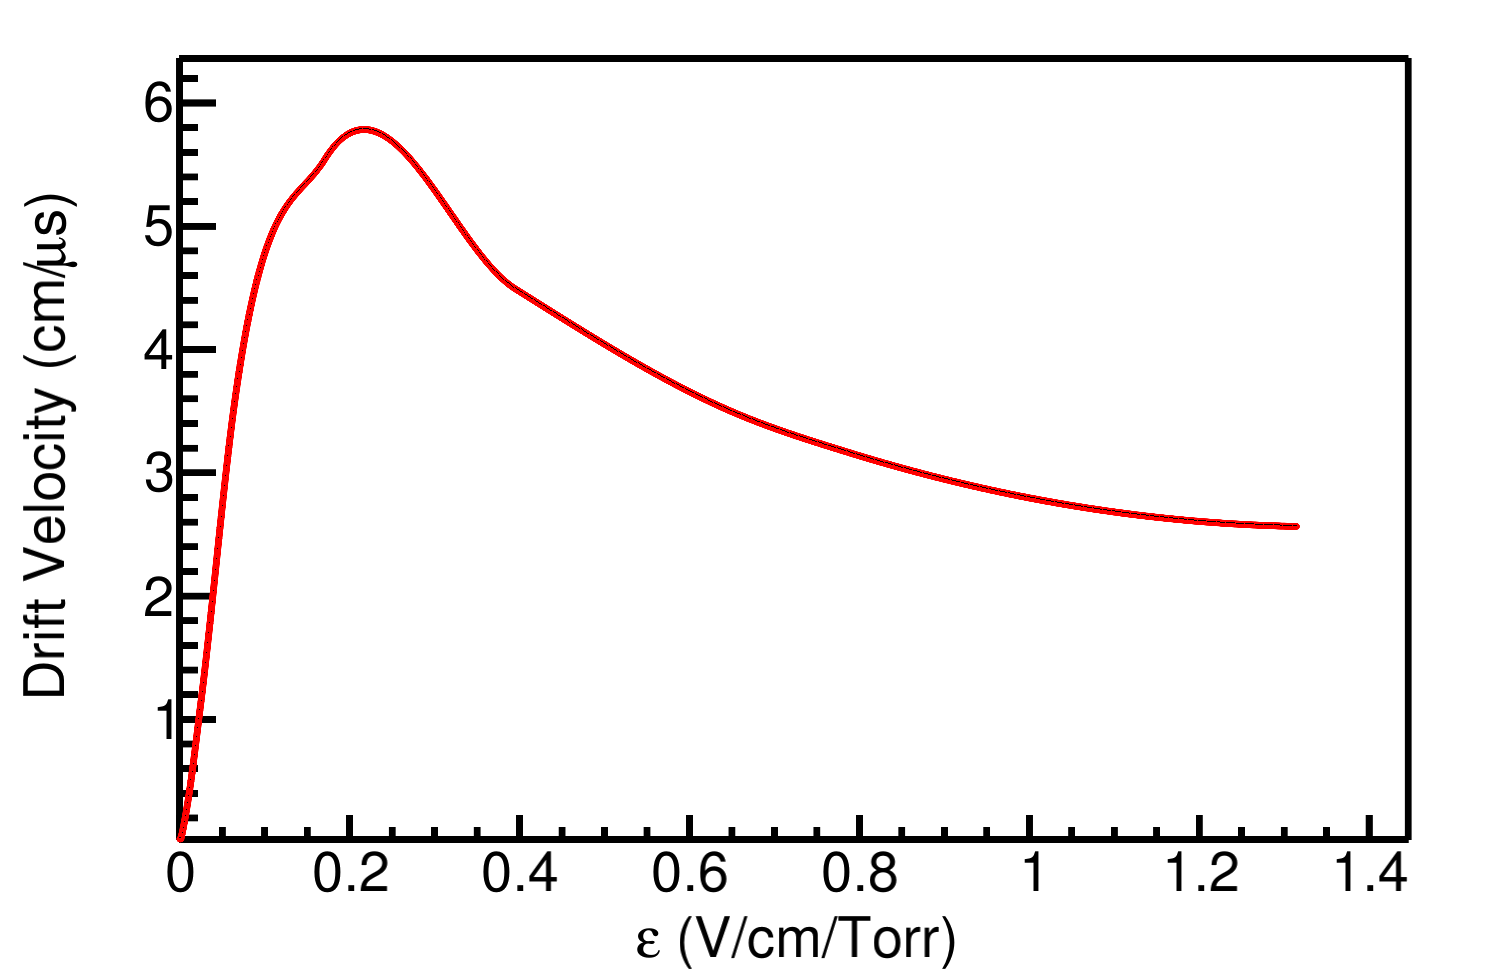
\includegraphics[width=\linewidth]{driftvel.png}
\caption{Drift velocity of electrons in P10 gas.}
\label{fig:driftvel}
\end{figure}

\begin{figure}
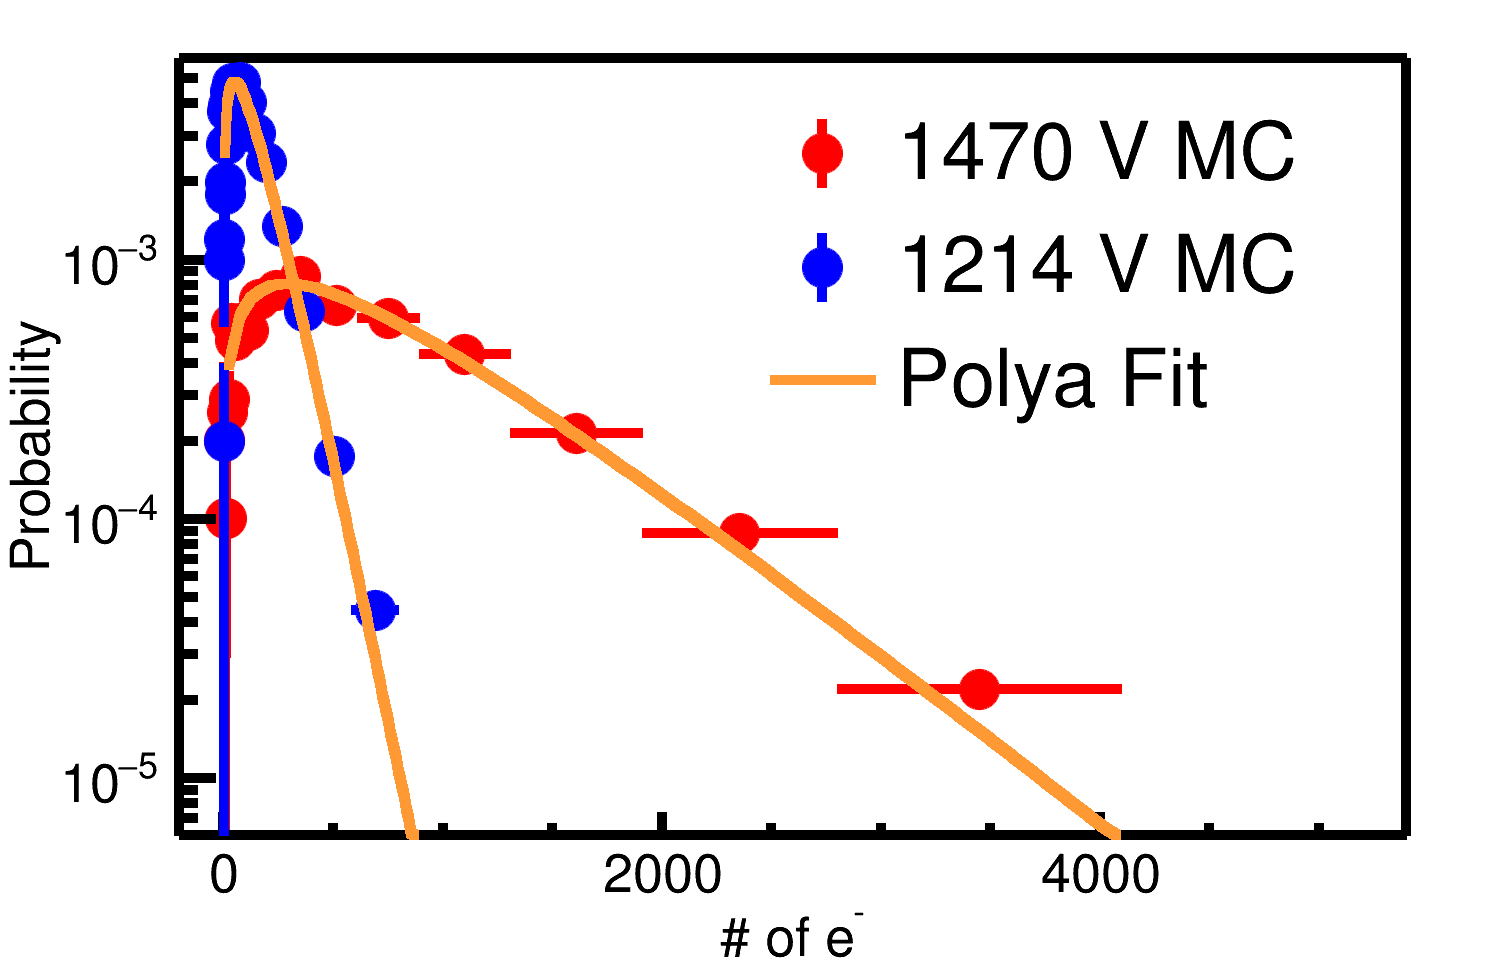
\includegraphics[width=\linewidth]{gain.png}
\caption{Number of electrons produced in a single avalanche on an anode wire. Two different voltages were simulated using Garfield++ at 1470 $V$ and 1214 $V$. The expected Polya distribution fit is also given in yellow.}
\label{fig:anodegain}
\end{figure}

\begin{table}[!htp] % not just 'h!'
\centering % not a center environment
\begin{tabular}{
  @{}
  l
  S[table-format=1.2]
  S[table-format=1.2]
  S[table-format=1.2]
  S[table-format=1.2]
  S[table-format=5.2]
  S[table-format=5.2]
  @{}
}
\toprule
Gas properties &
 {$\sigma_{t}$} &
 {$\sigma_{l}$} &
 {$v_{d}$} &
 {$v_{i}$}  &
 {$G_{h}$} &
 {$G_{l}$} \\
&
  {($\si{\centi\meter}^{-1/2}$)} &
  {($\si{\centi\meter}^{-1/2}$)} &
  {(\si{\centi\meter\per\micro\second})} &
 {(\si{\centi\meter\per\micro\second})} \\

\midrule
\phantom{abc}   &.024   &.034  &5.43  &  \num{2.05e-4} &  903   &150     \\
\bottomrule
\end{tabular}

\caption{}
\label{tb:gasprop}
\end{table}


Add table for gas diffusion 


\section{Ancillary Detectors }
\subsection{Kyoto Multiplicity Trigger}
\subsection{Krakow ?????? (KATANA)}

\section{Radio Isotope Beam Factory (RIBF) Facility }
Cyclotron facility overview.
Samurai line overview.
Beam line element overview.
Big rips beam PID. reference 


\section{S$\pi$RIT at RIBF}
Picture of setup. 




SAMURAI (Superconducting Analyzer for Multi-particles from Radioisotope beams) is a large-acceptance multi-particle spectrometer for radioactive-beam experiments.
\begin{figure}[H]
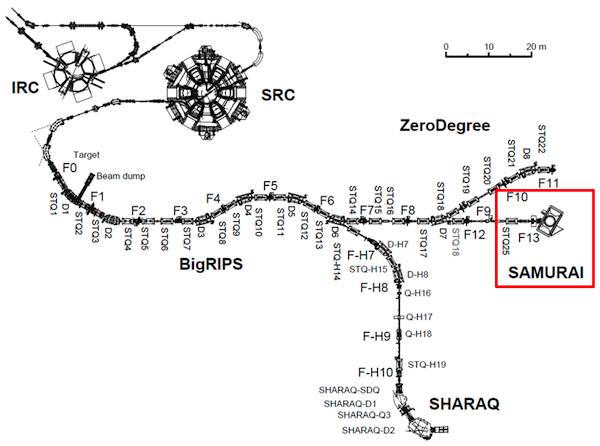
\includegraphics[width=\linewidth]{SAMURAI-beamline.png}
\caption{Overview of the RIBF, BigRIPS, and SAMURAI beamline.}
\label{fig:sambl}
\end{figure}

\section{Experimental Setup}

\section{Trigger Condition}
How it was made using kyoto krakow

\section{Collision Data Taken}

